\documentclass[xcolor=table]{beamer}

\usepackage[french]{babel}
\usepackage[latin1]{inputenc}
\usepackage[normalem]{ulem}
\usepackage[T1]{fontenc}
\usepackage{fancyhdr}   %% Pour la gestion des num�ros de page
\usepackage{graphicx}
\usepackage{amsmath}
\usepackage{mathrsfs}
\usepackage{amsfonts}
\usepackage{palatino}        %% Palatino fonts
\usepackage{mathptm}        %% PostScript Type 1 math fonts
\usepackage{dsfont} %% Pour mathds
\usepackage{color}
%%\usepackage{pstricks}
\usepackage{xmpmulti}
\usepackage{hyperref}
\usepackage{multimedia}
\usepackage{multirow}
%\usepackage[table]{xcolor}
\usepackage{fourier-orns}
\usepackage{subfigure}
\usepackage{tikz}

\DeclareMathAlphabet{\mathpzc}{OT1}{pzc}{m}{it}

\definecolor{vert}{rgb}{0.07,0.7,0.00}
\definecolor{gris}{gray}{0.70}
\definecolor{gris2}{gray}{0.95}
\definecolor{bleu}{rgb}{0.19,0.19,0.68}

%table setting
\newcommand\T{\rule{0pt}{2.6ex}}
\newcommand\B{\rule[-1.2ex]{0pt}{0pt}}
\renewcommand{\thesubfigure}{\thefigure.\arabic{subfigure}}

\usetheme{allee_marine} %voir fichier beaerthemeallee_marine.sty   ==> \usetheme{allee_marine}


%%%%%%%%%%%%%%%%%%%%%%%%%% Pr�sentation du document %%%%%%%%%%%%%%%%%%%%%%%%%%
\title[Master 1 Project]{Pr�sentation 29/05/2015}
\author[Etienne CAILLAUD, Thomas LE BRIS, Ibrahima GUEYE, Ga�tan ADIER]{\textbf{Etienne CAILLAUD, Thomas LE BRIS, Ibrahima GUEYE, Ga�tan ADIER}}
\institute [XLIM-SIC UMR CNRS 7252]{\textbf{XLIM-SIC Laboratory UMR CNRS 7252, Poitiers, France}}
\date{}

%%%%%%%%%%%%%%%%%%%%%%% Num�ro de pages en bas � gauche %%%%%%%%%%%%%%%%%%%%%%
\addtobeamertemplate{footline}{\color{blue}\hfill\insertframenumber/\inserttotalframenumber}

\pgfdeclareimage[height=96mm,width=128mm]{nombidon}{mood_eye_light}
\setbeamertemplate{background}{\pgfuseimage{nombidon}}

\pgfdeclareimage[height=96mm,width=128mm]{nombidon2}{mood_eye_light}
\setbeamertemplate{background}{\pgfuseimage{nombidon2}}

%%----------------------------------------------------------------------------
%% A chaque d�but de sous-section : g�n�re une table des mati�res
%%----------------------------------------------------------------------------
\AtBeginSection[]
{
   \setbeamertemplate{background}{\pgfuseimage{nombidon}}
   \begin{frame}<beamer>
    \frametitle{Outline}
    \tableofcontents[currentsection, hideallsubsections] %% affiche la section courante et les autres en gris�, masque les sous-sections
   \end{frame}
  \setbeamertemplate{background}{\pgfuseimage{nombidon2}}
}

\AtBeginSubsection[]
{
  \setbeamertemplate{background}{\pgfuseimage{nombidon}}
  \begin{frame}<beamer>
    \tableofcontents[sectionstyle=show/shaded,subsectionstyle=show/shaded/hide, subsubsectionstyle =hide]
  \end{frame}
   \setbeamertemplate{background}{\pgfuseimage{nombidon2}}
}

\AtBeginSubsubsection[]
{
  \setbeamertemplate{background}{\pgfuseimage{nombidon}}
  \begin{frame}<beamer>
    \tableofcontents[sectionstyle=show/shaded,subsectionstyle=show/shaded/hide,subsubsectionstyle =show/shaded/hide]
  \end{frame}
   \setbeamertemplate{background}{\pgfuseimage{nombidon2}}
}


%%%%%%%%%%%%%%%%%%%%%%%%%%%%%%%%%%%%%%%%%%%%%%%%%%%%%%%%%%%%%%%%%%%%%%%%%%%%%%
%%%%%%%%%%%%%%%%%%%%%%%%%%%%                       %%%%%%%%%%%%%%%%%%%%%%%%%%%
%%%%%%%%%%%%%%%%%%%%%%%%%%     D�BUT DU DOCUMENT     %%%%%%%%%%%%%%%%%%%%%%%%%
%%%%%%%%%%%%%%%%%%%%%%%%%%%%                       %%%%%%%%%%%%%%%%%%%%%%%%%%%
%%%%%%%%%%%%%%%%%%%%%%%%%%%%%%%%%%%%%%%%%%%%%%%%%%%%%%%%%%%%%%%%%%%%%%%%%%%%%%
\begin{document}
\graphicspath{{images/}}
\setbeamercolor{block title example}{bg = gray}

\begin{frame}
    \vspace{-1.5cm}
    \begin{tikzpicture}[remember picture,overlay]
        \node[xshift=0cm, above=8.6cm] at (current page.south west)
        {
\includegraphics[width=40cm,height=0.9cm]{cache_titre.png}};
        \node[xshift=2cm, above=2.8cm] at (current page.south west)
        {
\includegraphics[height=1.5cm]{Xlim.png}};
        \node[xshift=11cm, above=3cm] at (current page.south west)
        {
\includegraphics[height=1cm]{logo_une.jpg}};
        \node[xshift=6.5cm, above=0.7cm] at (current page.south west)
        {
\includegraphics[height=1.6cm]{Lifeclef.png}};
    \end{tikzpicture}
    \titlepage
\end{frame}

%%%%%%%%%%%%%%%%%%%%%%%%%%%%%%%%%%%%%%%%%%%%%%%%%%%%%%%%%%%%%%%%%%%%%%%%%%%%%%%%%%%%%%%%%%%%%%%%%%%%%
%%%%%%%%%%%                        D�but de la pr�sentation                       			 %%%%%%%%
%%%%%%%%%%%%%%%%%%%%%%%%%%%%%%%%%%%%%%%%%%%%%%%%%%%%%%%%%%%%%%%%%%%%%%%%%%%%%%%%%%%%%%%%%%%%%%%%%%%%%
\section{Process flow}
%%-----------------------------------------------------------------------------------------
\begin{frame} \frametitle{Presentation de la fonction}
%%-----------------------------------------------------------------------------------------
  \vspace{0.2cm}
    \begin{itemize}
        \item Fonction permettant la gestion complete de tout les autres fonctions
    \end{itemize}
    \begin{block}{Prototype de la fonction}
        def descript (path_work, name_desc, path_images, nb_class, nb_images = "ALL", start_img = 1):
    \end{block}
    \begin{itemize}
        \item Permet la creation de l'arborescence.
        \item modification d'une boucle pour passer d'un descripteur a un autre.
    \end{itemize}
\end{frame}


%%-----------------------------------------------------------------------------------------

\begin{frame} \frametitle{Arborescence}
%%-----------------------------------------------------------------------------------------
    \begin{figure}[ht]
        \centering
        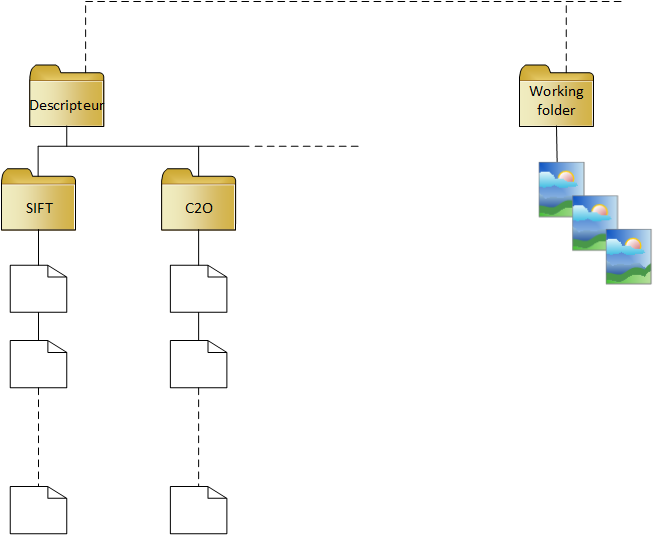
\includegraphics[scale=0.35]{arborescence.png}
        \caption{Arborescence issue par le programme}
        \label{fig:img_arbo}
    \end{figure}

\end{frame}
%%-----------------------------------------------------------------------------------------

\section{Descripteurs}
%%-----------------------------------------------------------------------------------------
\begin{frame} \frametitle{SIFT (1/?)}
%%-----------------------------------------------------------------------------------------
   \begin{itemize}

   \end{itemize}
\end{frame}
%%-----------------------------------------------------------------------------------------

\begin{frame} \frametitle{C$_2$O (1/?)}
%%-----------------------------------------------------------------------------------------
   \begin{itemize}

   \end{itemize}
\end{frame}
%%-----------------------------------------------------------------------------------------

\section{Classification}
%%-----------------------------------------------------------------------------------------
\begin{frame} \frametitle{Principe}
%%-----------------------------------------------------------------------------------------
   \begin{itemize}
        \item Definir l'ensemble des descripteur pour toutes les images.
        \item Calcul du K-Means.
        \item Creation de la signature pour toutes les images.
        \item Calcul de distance entre les diff�rentes signature ($\chi^2$, Euclidienne).
   \end{itemize}
   \begin{block}{Equation K-Means}
        \centering
        \sum\sum\parallel x_j - u_i \parallel ^2
    \end{block}
\end{frame}
%%-----------------------------------------------------------------------------------------

\begin{frame} \frametitle{Resultats}
%%-----------------------------------------------------------------------------------------
   \begin{figure}[ht]
        \centering
        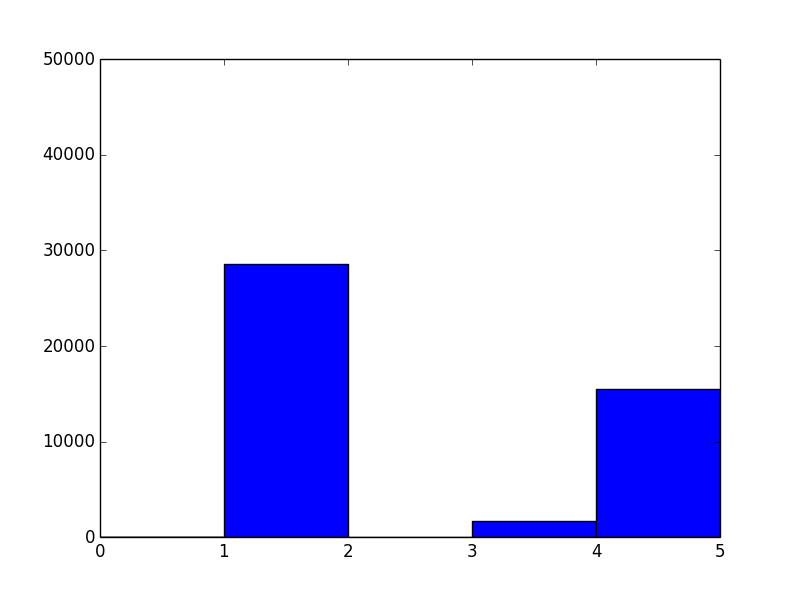
\includegraphics[scale=0.35]{histo1.png}
        \caption{Histogramme repr�sentant l'ensemble des images}
        \label{fig:img_arbo}
    \end{figure}
\end{frame}
%%-----------------------------------------------------------------------------------------

\section{XML/TXT}
%%-----------------------------------------------------------------------------------------
\begin{frame} \frametitle{Formalisation des documents}
%%-----------------------------------------------------------------------------------------
   \begin{itemize}
        \item sauvegarde des keypoints
        \item r�sultat du run : <ObservationId;ClassId;rank;score>
        \item optionnel : test$_$image$_$name.jpg;ClassId;rank;score
        \item calcul du score : S=$\frac{1}{U}$ $\sum_{u=1}^{U}\frac{1}{P_{u}}$ $\sum_{p=1}^{P_u}S_{u,p}$
        
   \end{itemize}
\end{frame}
%%-----------------------------------------------------------------------------------------

\section{Parallelisation}
%%-----------------------------------------------------------------------------------------
\begin{frame} \frametitle{Justification du choix}
%%-----------------------------------------------------------------------------------------
   \begin{itemize}

   \end{itemize}
\end{frame}
%%-----------------------------------------------------------------------------------------

\begin{frame} \frametitle{Application}
%%-----------------------------------------------------------------------------------------
   \begin{itemize}

   \end{itemize}
\end{frame}
%%-----------------------------------------------------------------------------------------


\section{HULK}
%%-----------------------------------------------------------------------------------------
\begin{frame} \frametitle{Presentation de la documentation}
%%-----------------------------------------------------------------------------------------
   \begin{itemize}

   \end{itemize}
\end{frame}
%%-----------------------------------------------------------------------------------------

\section{Working Paper}
%%-----------------------------------------------------------------------------------------
\begin{frame} \frametitle{Attente du CLEF}
%%-----------------------------------------------------------------------------------------
   \begin{itemize}
        \item tasks performed
        \item main objectives of experiments
        \item approach(es) used and progress beyond state-of-the-art
        \item resources employed
        \item results obtained
        \item analysis of the results
        \item perspectives for future work
   \end{itemize}
\end{frame}
%%-----------------------------------------------------------------------------------------


\end{document}


